\documentclass[10pt]{article}

\usepackage{amsfonts,amssymb}
\usepackage[utf8]{inputenc}
\usepackage[english,russian]{babel}
\usepackage{graphicx}
\usepackage{mathtools}
\usepackage{multicol}
\usepackage{ textcomp }
\usepackage[colorlinks,urlcolor=blue]{hyperref}

\newcommand{\argmin}{\mathop{\rm arg\,min}\limits}
\newcommand{\argmax}{\mathop{\rm arg\,max}\limits}
\newcommand{\sign}{\mathop{\rm sign}\limits}
\newcommand{\cond}{\mspace{3mu}{|}\mspace{3mu}}
\def\RR{\mathbb{R}}
\def\XX{\mathbb{X}}
\def\EE{\mathbb{E}}
\def\NN{\mathcal{N}}
\def\LL{\mathcal{L}}
\def\YY{\mathbb{Y}}

\textheight=220mm
\textwidth=160mm

\title{Школа анализа данных\\ Восстановление зависимостей \\Домашнее задание №4}
\author{Кошман Дмитрий}
\date{}

\begin{document}
	
	
	\voffset=-20mm
	\hoffset=-17mm
	\font\Got=eufm10 scaled\magstep2 \font\Got=eufm10
	
	
	\maketitle
	
\bigskip

\textbf{Задача 1}

\medskip

Вывести формулу для оценки качества построения гребневой регрессии методом скользящего контроля:

$$ \hat{S} =  \frac{1}{l} \sum_{i=1}^{l} \left( \frac{y_i - t_i}{1-h_{ii}} \right)^2,$$

\begin{center}
	где $ h= F(F^TF +\lambda I)^{-1} F^T, \medspace t =hy,\medspace F\in \mathbb{R} ^{l\times n}, \medspace y\in \mathbb{R} ^{l} $
\end{center}

\medskip

Предсказания гребневой регрессии в точке $X$ выглядит как $y^* =Xw^* $, где

$$w^* =  \argmin_w  \left(||Fw - y||^2_2 + \lambda||w||^2_2 \right); F,y -\text{обучающая выборка}$$

Выразим $w^*$, посчитав градиент:

\medskip

$\left[ D_{w^*}(|Fw - y|^2 + \lambda|w|^2) \right](h) = \left[ D_{w^*}(\langle Fw - y,Fw - y\rangle +\lambda \langle w, w\rangle) \right](h) = $\\

$2\langle Fw^* - y,Fh\rangle + 2\lambda\langle w^*, h\rangle = 2\langle F^T(Fw^* - y) +\lambda w^* ,h\rangle =  \langle \nabla_w, h \rangle$,\\

$\nabla_w =2(F^T(Fw^* - y) +\lambda w^*) = 0$\\

$(F^TF + \lambda I)w^* = F^Ty$\\

$w^* = (F^TF + \lambda I)^{-1}F^Ty $\\

В случае LOO кросс валидации, модель обучается на подвыборках $\hat{F}_i\in \mathbb{R} ^{l-1\times n}, \medspace \hat{y}_i\in \mathbb{R} ^{l-1}$, которые образованы поочередным выкидыванием элементов из обучающей выборки. Тогда потери на одной кросс валидации равны\\

$ (y^*_i - y_i)^2 = (F_iw^*_i - y_i)^2 = (F_i(\hat{F}_i^T\hat{F}_i + \lambda I)^{-1}\hat{F}_i^T\hat{y}_i - y_i)^2$,\\

где $F_i$ -- $i$-ая строчка.

Заметим, что \\

$(\hat{F}_i^T\hat{F}_i)_{jk} = \sum_{t} F^T_{jt}F_{tk} - F^T_{ji}F_{ik} = (F^TF)_{jk} - (F_i^TF_i)_{jk} \Rightarrow \hat{F}_i^T\hat{F}_i = F^TF - F_i^TF_i$\\

$(\hat{F}_i^T\hat{y}_i)_j = (\hat{F}_i^T)_j\hat{y}_i = \sum_{t} F^T_{jt}y_t - F^T_{ji}y_i = (F^Ty)_j - (F_i^Ty_i)_j \Rightarrow \hat{F}_i^T\hat{y}_i =  F^Ty - F_i^Ty_i$\\

Тогда \\

$(y^*_i - y_i)^2 =\left(F_i(F^TF - F_i^TF_i + \lambda I)^{-1}(F^Ty - F_i^Ty_i) - y_i\right)^2 $\\

Выразим $t_i, h_{ii}$:\\

$h_{ii} = (F(F^TF +\lambda I)^{-1} F^T)_{ii} = F_i(F^TF +\lambda I)^{-1} F_i^T$,\\

$t_i = (hy)_i=h_i y =(F(F^TF +\lambda I)^{-1} F^T)_i y = F_i(F^TF +\lambda I)^{-1} F^Ty$\\

Пусть $A = (F^TF +\lambda I)^{-1}, \medspace B = (F^TF - F_i^TF_i + \lambda I)^{-1}$, тогда \\

$(y^*_i - y_i)^2 = \left( \frac{(1-h_{ii})(y^*_i - y_i) }{1-h_{ii}} \right)^2 = 
\left( \frac{(1- F_i AF_i^T)(F_iB(F^Ty-F_i^Ty_i) - y_i) }{1-h_{ii}} \right)^2=$\\

$\left( \frac{F_iB(F^Ty-F_i^Ty_i) - y_i- F_i AF_i^TF_iB(F^Ty-F_i^Ty_i) +F_i AF_i^T y_i }{1-h_{ii}} \right)^2$\\

Заметим, что $F_i^TF_i = A^{-1} - B^{-1} $, тогда\\

$(y^*_i - y_i)^2 = \left( \frac{F_iB(F^Ty-F_i^Ty_i) - y_i- F_i A(A^{-1} - B^{-1})B(F^Ty-F_i^Ty_i) +F_i AF_i^T y_i }{1-h_{ii}} \right)^2$=\\

$\left( \frac{(F_iB(F^Ty-F_i^Ty_i) - y_i- F_i B(F^Ty-F_i^Ty_i) + F_i A(F^Ty-F_i^Ty_i) +F_i AF_i^T y_i }{1-h_{ii}} \right)^2$=\\

$\left( \frac{F_i AF^Ty -y_i }{1-h_{ii}} \right)^2$= $\left( \frac{t_i -y_i }{1-h_{ii}} \right)^2$\\

Взяв среднее по всем подвыборкам, получим исходную формулу.

\bigskip

\textbf{Задача 2}

\medskip

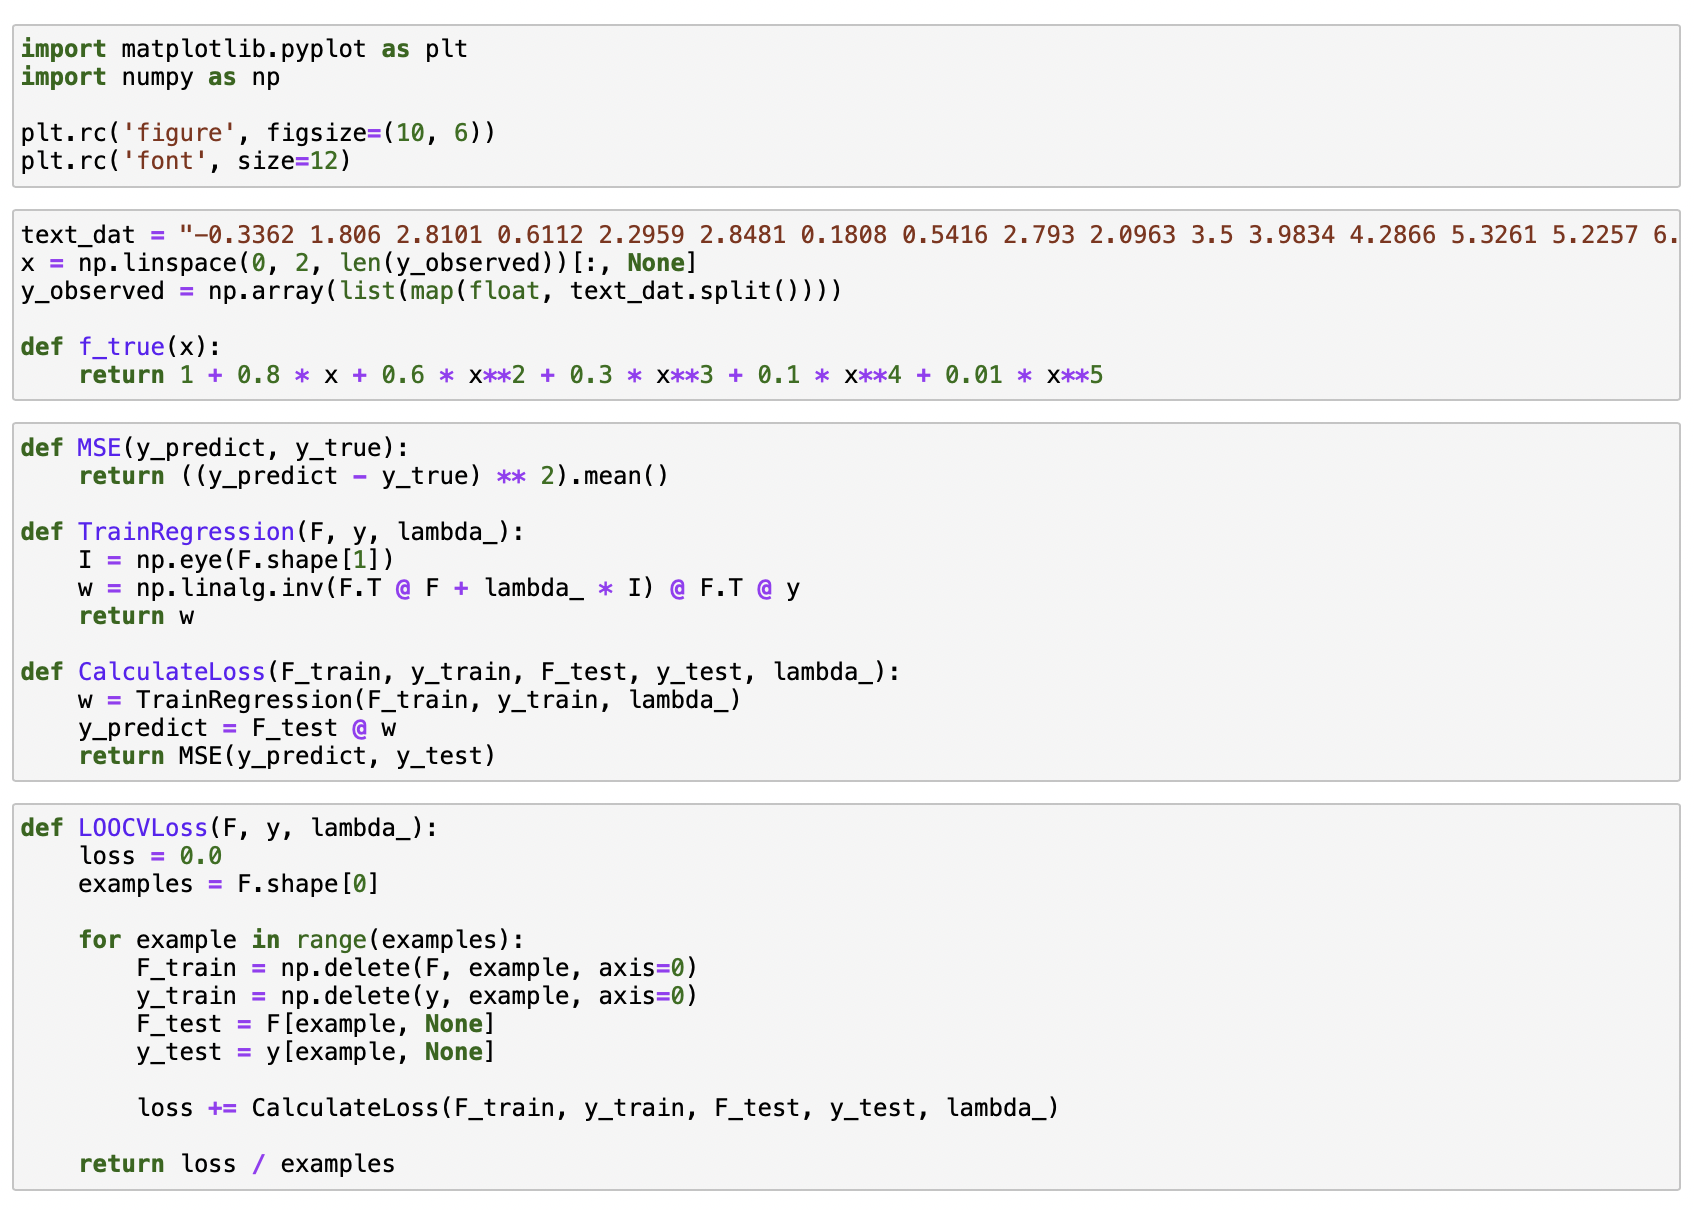
\includegraphics[width=.8\textwidth]{Screenshot 2022-04-05 at 16.44.08}\\
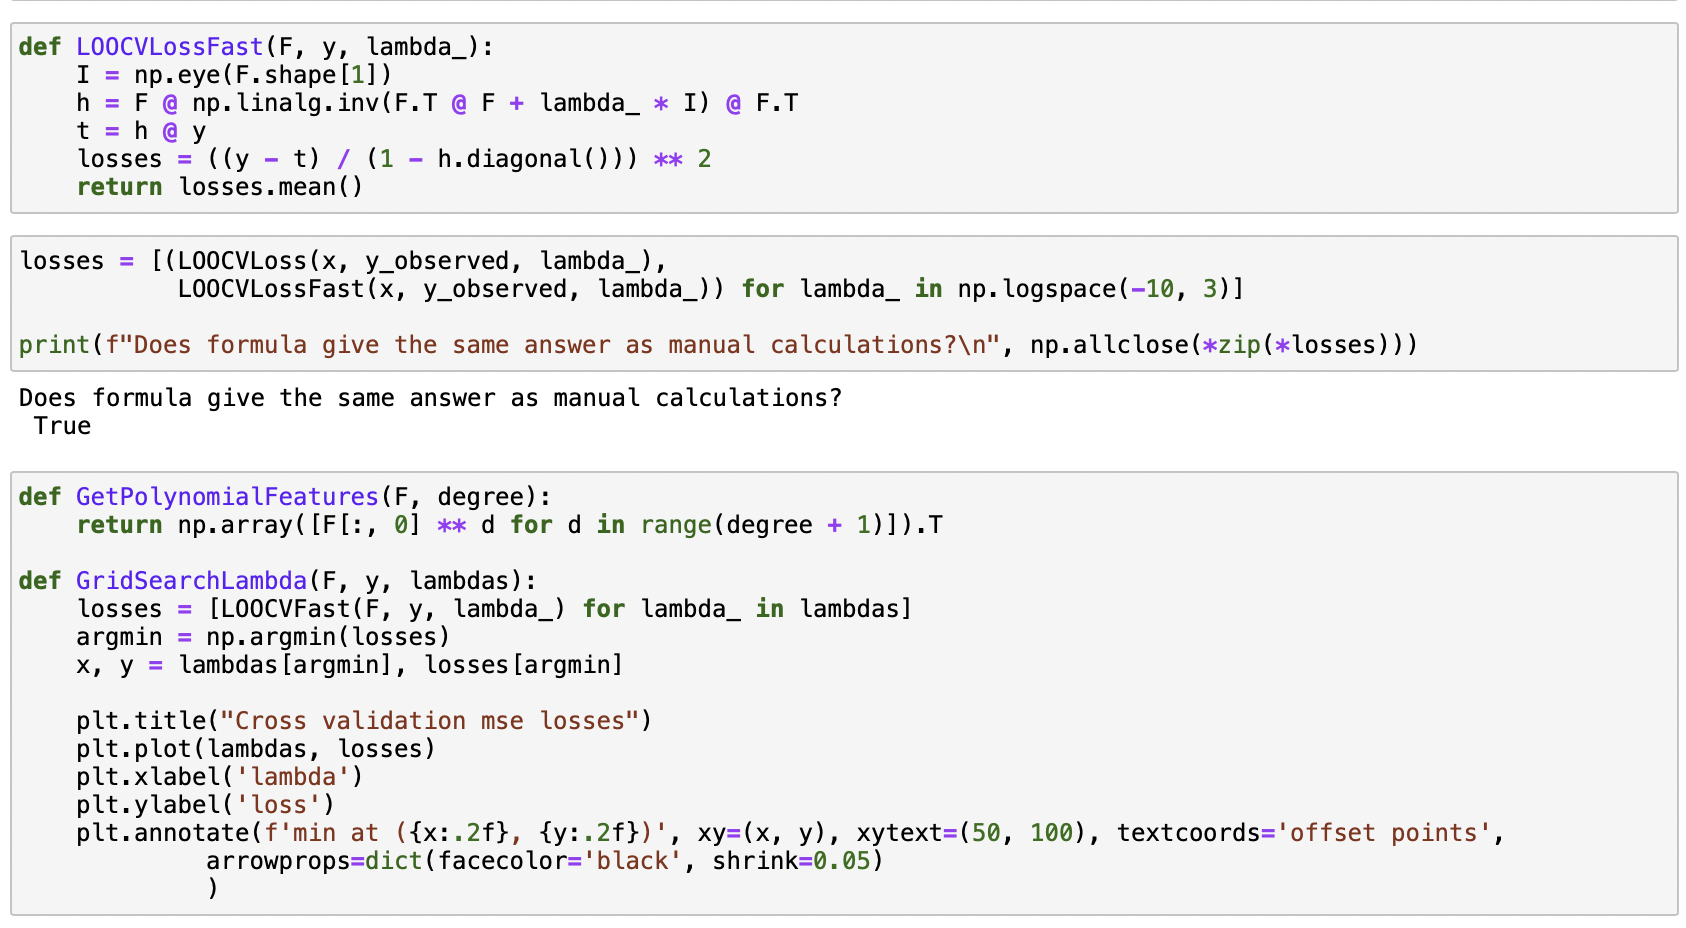
\includegraphics[width=.8\textwidth]{Screenshot 2022-04-05 at 16.50.35}\\
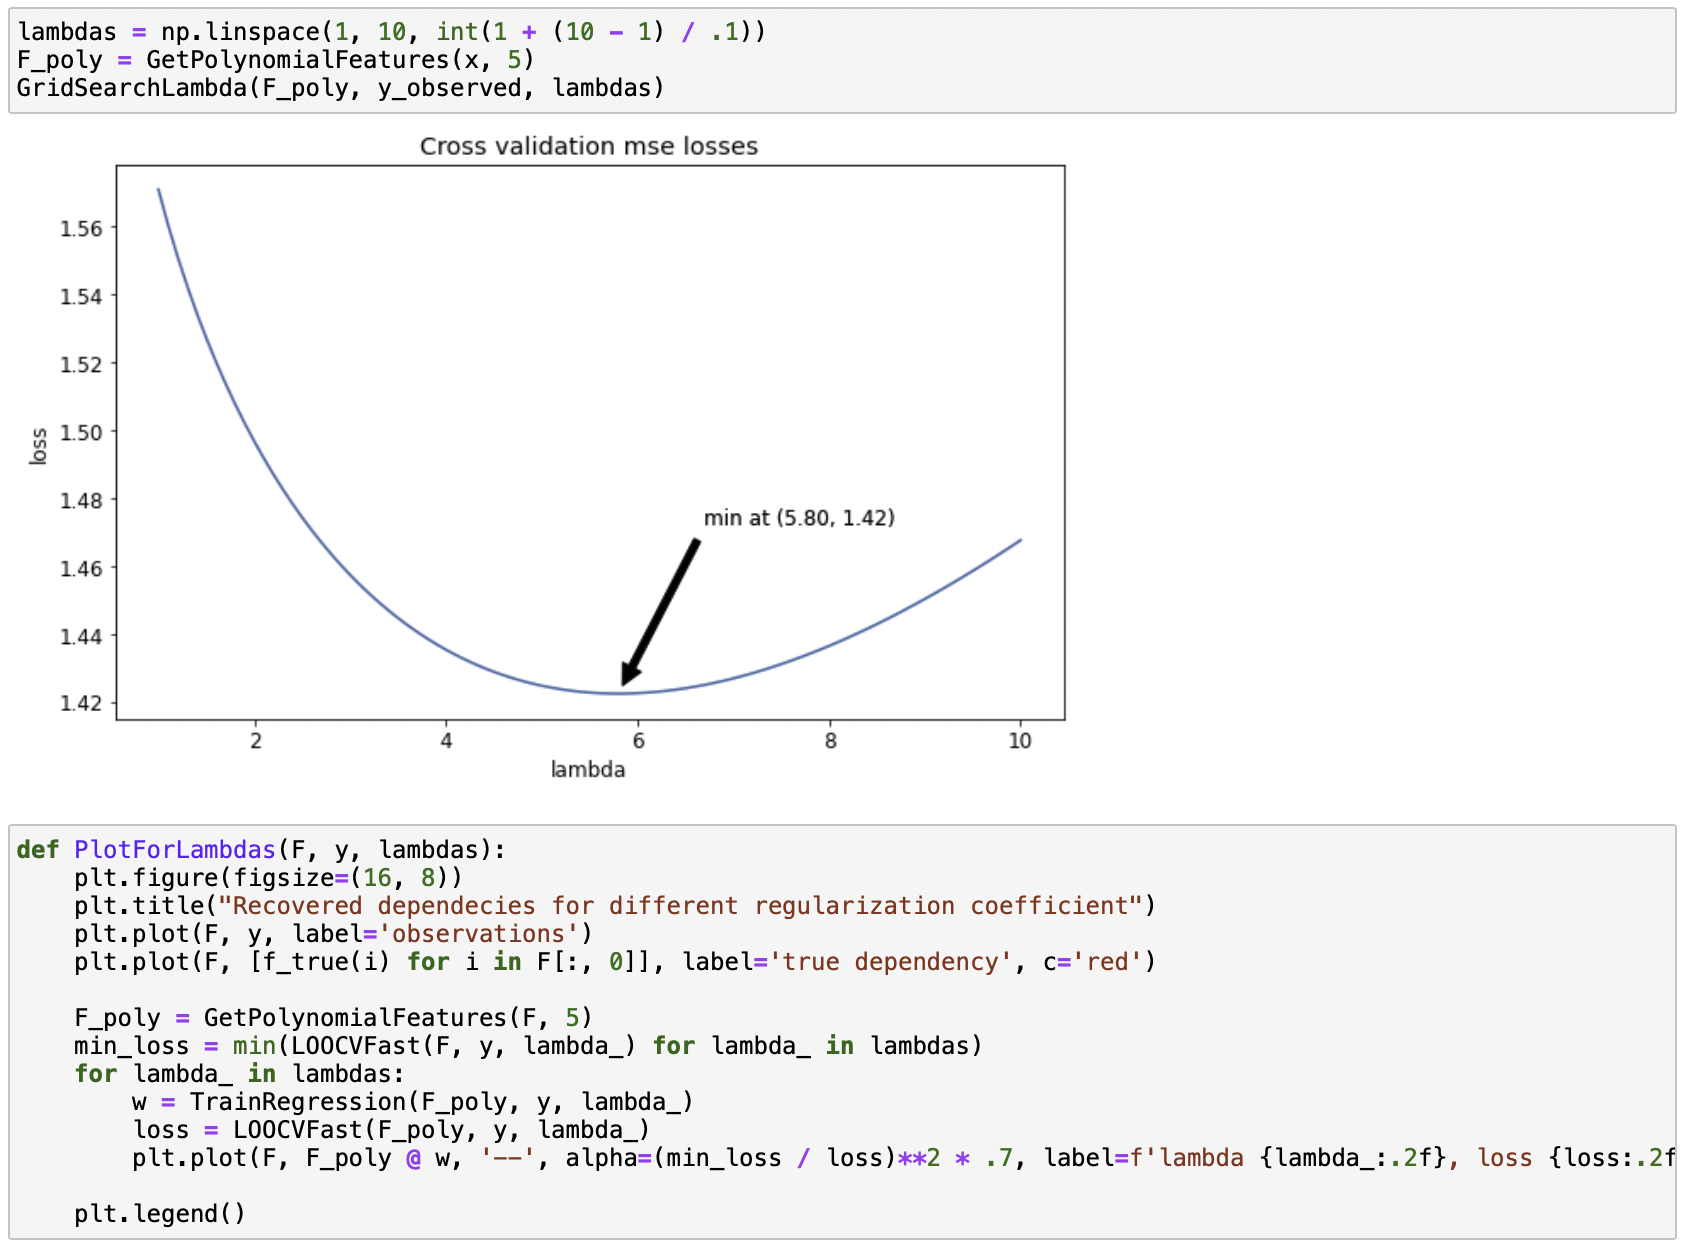
\includegraphics[width=.8\textwidth]{Screenshot 2022-04-05 at 16.50.54}\\
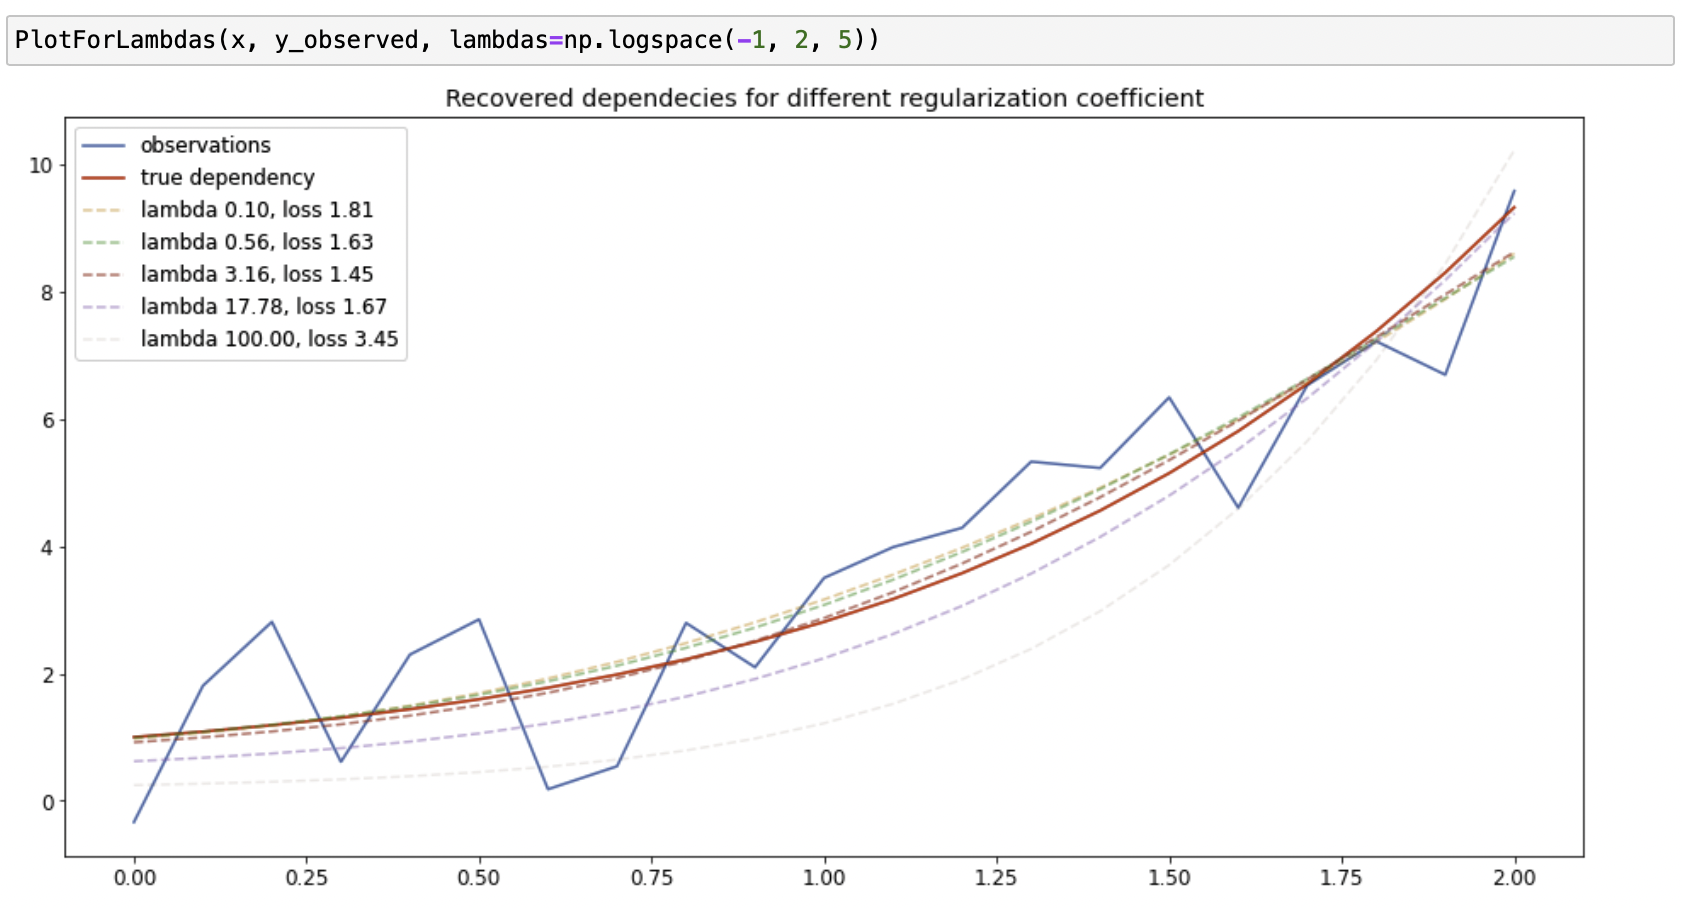
\includegraphics[width=.8\textwidth]{Screenshot 2022-04-05 at 16.51.06}\\

\bigskip


\textbf{Задача 3}

\medskip

$y = Xa + \epsilon, \medspace \epsilon \sim \mathcal{N}(0, I), \medspace a \sim Laplace(0, I)$\\

$\hat{a}_{MAP} - ?$\\

$\hat{a}_{MAP}(X, y) = \underset{a}{\argmax} \thinspace p_\epsilon(\epsilon| a)p_a(a)=\underset{a}{\argmax} \thinspace p_\epsilon(y - Xa)p_a(a)=$\\

$\underset{a}{\argmax} \thinspace \prod_{i} \frac{1}{\sqrt{2\pi}} \exp\{-\frac{(y_i - X_ia)^2}{2}\}\prod_{j}\exp\{-\frac{|a_j|}{2}\} =$\\

$\underset{a}{\argmax} \thinspace\log \prod_{ij}\exp\{-\frac{(y_i - X_ia)^2}{2}\}\exp\{-\frac{|a_j|}{2}\} =$\\

$\underset{a}{\argmax} \thinspace \sum_{ij} -(y_i - X_ia)^2-|a_j| =$\\

$\underset{a}{\argmin} \thinspace \sum_{i} (y_i - X_ia)^2 + |a_i| =$\\

$\underset{a}{\argmin} \thinspace  ||y - Xa||_2^2 + ||a||_1 $\\

Заметим, что сумма норм - выпуклая функция, значит минимум существует и единственнен. Явного выражения для $\hat{a}_{MAP}$ не существует, но можно находить его численно градиентным спуском, доопределяя градиент при попадании на координатные оси:\\

$\left[ D_{a^*}(||y - Xa||_2^2 + ||a||_1) \right](h) = 2\langle X^T(Xa^* - y) + \sign (a^*) ,h\rangle = \langle \nabla_a, h \rangle$\\

$\nabla_a = 2X^T(Xa^* - y) + \sign (a^*) $\\

Если же $a \sim \mathcal{N}(0, I)$, то\\

$\hat{a}_{MAP}(X, y) = \underset{a}{\argmin} \thinspace  ||y - Xa||_2^2 + ||a||^2_2 =
( X^TX + I)^{-1}  X^Ty$\\





\end{document}

